\subsection{Observer (\textit{o Dependents, Publish-Subscribe})}
\label{observer}

\textbf{Scopo}: Comportamentale \\
\textbf{Raggio d'azione}: Oggetti

\paragraph{Definizione} Il pattern Observer permette di definire una dipendenza uno a molti tra oggetti, in modo tale che se un oggetto cambia il suo stato, tutti gli oggetti dipendenti da questo siano notificati e aggiornati automaticamente.

\begin{figure}[H]
    \centering
    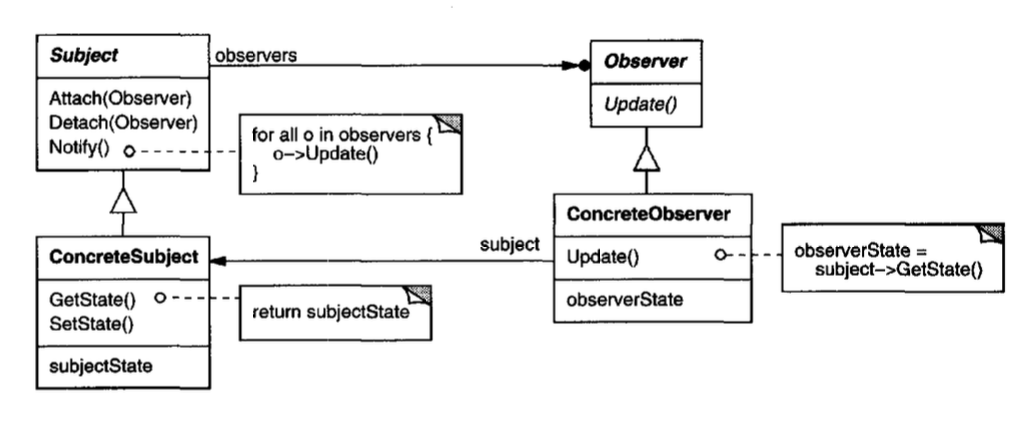
\includegraphics[width=1\linewidth]{assets/pattern/observer/observer-struttura.png}
\end{figure}

\paragraph{Struttura} Il pattern è composto da:
\begin{itemize}
    \item \textbf{Subject}: conosce i propri osservatori; un numero qualunque di oggetti Observer può osservare un soggetto. Fornisce un’interfaccia per registrare e cancellare le registrazioni degli oggetti Observer. 
    \item \textbf{Observer}: fornisce un’interfaccia di notifica per gli oggetti a cui devono essere notificati i cambiamenti nel Subject. 
    \item \textbf{ConcreteSubject}: contiene lo stato a cui gli oggetti 
     ConcreteObserver sono interessati. Inoltra una notifica ai suoi Observer quando il proprio stato si modifica. 
    \item \textbf{ConcreteObserver}: memorizza un riferimento a un oggetto ConcreteSubject oppure ottiene dinamicamente il riferimento all’oggetto Subject da cui ha origine la notifica in caso in esso cui osservi più Subject. Contiene informazioni che devono essere sincronizzate con lo/gli stato/i del/i Subject. Implementa l’interfaccia Observer per ricevere le notifiche del Subject.
\end{itemize}

\begin{figure}[H]
    \centering
    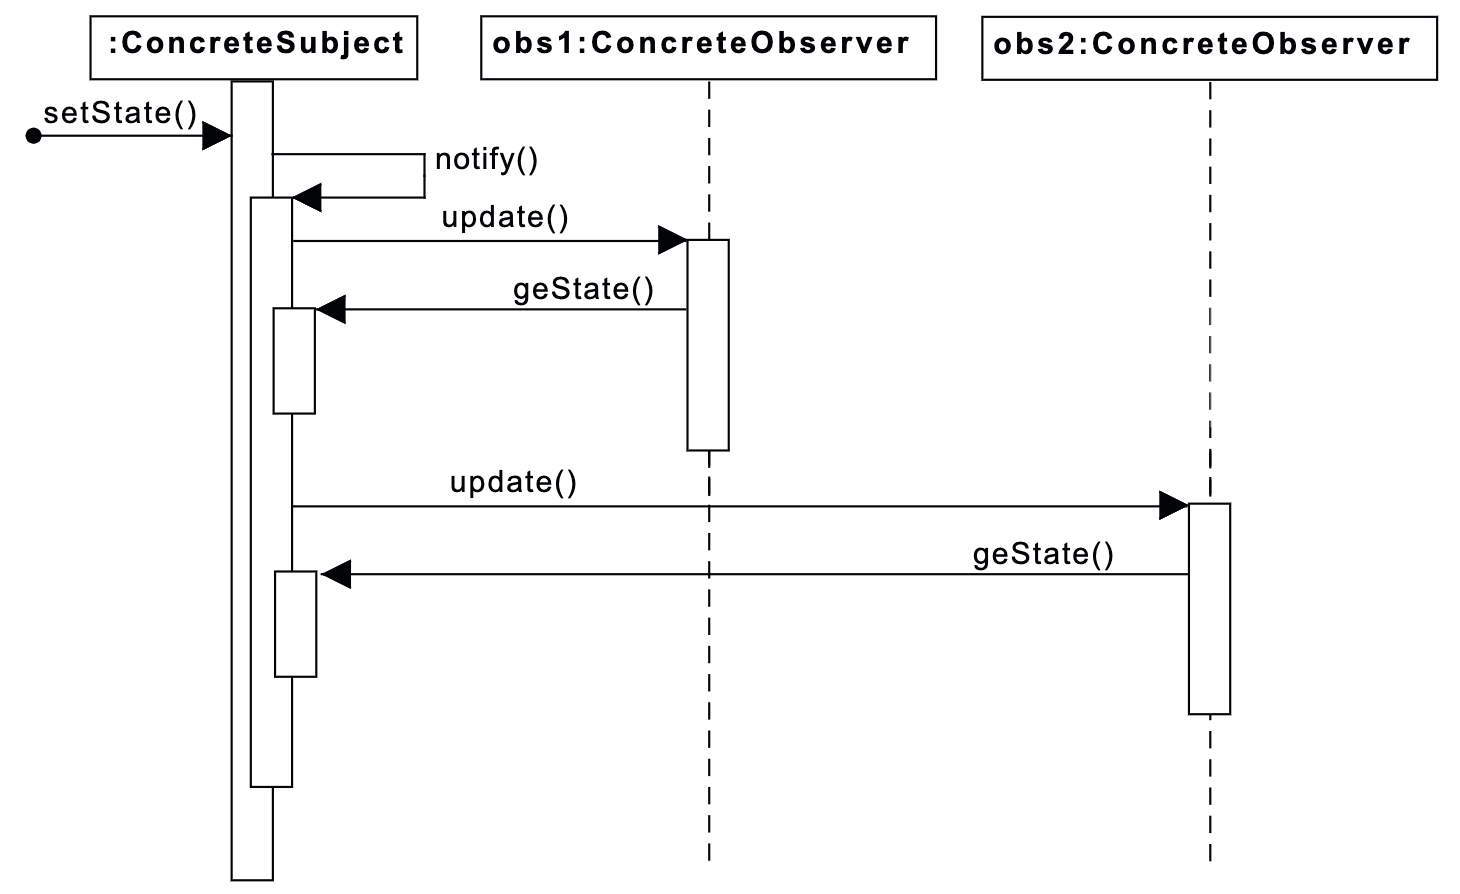
\includegraphics[width=1\linewidth]{assets/pattern/observer/observer-activity.png}
\end{figure}

\paragraph{Interazioni} ConcreteSubject notifica i propri Observer quando avviene un cambiamento che potrebbe rendere il loro stato non inconsistente rispetto al proprio. Dopo essere stato informato di un cambiamento nel ConcreteSubject, un osservatore concreto può chiedere al Subject informazioni sul suo stato. ConcreteObserver usa questa informazione per riconciliare il suo stato con quello del subject.

\newpage